\documentclass[english]{../TexTemplate/thesis}
\usepackage[cpp]{../TexTemplate/mypackage}

\title{Week 3 - C/C++ Toolchain}
\author{Hongzheng Chen\qquad Yucheng Chen}
\date{Nov 29, 2019}
\headercontext{Week 3 - C/C++ Toolchain}

\begin{document}

\maketitle

Week 3's seminar is partly based on \href{https://cornell-ece2400.github.io/ece2400-docs/ece2400-sec2-c-basics/}{Cornell ECE 2400: Computer Systems Programming} lectured by Christopher Batten in Fall 2019.

\section{C/C++ Introduction}
As discussed in seminar, we use C and C++ as introductory languages for the following reasons:
\begin{itemize}
	\item High-performance: C/C++ is extremely fast and is widely used in HPC.
	\href{https://www.openmp.org/}{OpenMP} and \href{https://mpitutorial.com/tutorials/}{MPI} are two most commonly used parallel libraries based on C, which will be covered in your \emph{Parallel and Distributed Computing} course in Grade 2, \emph{Distributed Systems} in Grade 3, and \emph{High-Performance Computing} in Grade 3.
	Specific accelerators use C-like languages to program.
	For example, GPU uses \href{https://www.infoworld.com/article/3299703/what-is-cuda-parallel-programming-for-gpus.html}{CUDA} to program (\emph{Parallel and Distributed Computing}), and FPGA uses \href{https://www.doulos.com/knowhow/verilog_designers_guide/what_is_verilog/}{Verilog} to program (\emph{Digital Circuits} in Grade 1 and \emph{Computer Organization} in Grade 2), both of which are C language's extension.
	\item Fundamental: C/C++ is very close to the hardware, thus makes you better understand how the computer works.
	\emph{Operating Systems}, \emph{Computer Networking}, and \emph{Embedded Systems} in Grade 2 all require you have a good understanding of C.
	Otherwise, you can hardly make it work with assembly and correctly run on hardware.
	\item Influential: C/C++ influences many programming languages, including Java and C\#, as depicted in \href{https://exploring-data.com/vis/programming-languages-influence-network/}{Programming Languages Influence Network}.
	Thus, if you learn C/C++ well, you will easily understand the primitives of other languages.
\end{itemize}

Two introductory books about C and C++ are:
\begin{itemize}
	\item Brian Kernighan, Dennis Ritchie, \emph{The C Programming Language (2nd ed.)}, Prentice-Hall, 1988 (\href{https://book.douban.com/subject/1139336/}{Chinese version})
	\item Stanley B. Lippman, Josée Lajoie, Barbara E. Moo, \emph{C++ Primer (5th ed.)}, Objectwrite, 2012 (\href{https://book.douban.com/subject/25708312/}{Chinese version})
\end{itemize}

Please learn the theory of C/C++ carefully, since they may greatly influence your future courses.
About C language's basic theory, you can see \href{https://cornell-ece2400.github.io/ece2400-docs/ece2400-T01-intro-c/}{Topic 1: Introduction to C} of \emph{Cornell ECE 2400}, or refer to my Github \href{https://github.com/chhzh123/CS-Notes/tree/master/C-Programming}{notes}.

Also, pay more attention to the difference between C and C++.
C++ is NOT C plus STL.
C++ is more than that, with support to Object-Oriented Programming (OOP), templates and generic programming, and other modern language features.
All of these can be found in the \href{https://book.douban.com/subject/25708312/}{\emph{C++ Primer}} book.

\section{Stages of Compilation}
C language's compilation mainly consists of the four stages listed below.
You have to clearly know what these stages do, which will give you better understandings when you read papers or do projects about compilers or systems in the future.
I highly recommend you to read the \href{https://csapp.cs.cmu.edu/}{\emph{Computer Systems: A Programmer's Perspective (CS:APP)}} book, Chapter 1 of which gives the overview of computer system stack.
\begin{center}
\begin{tikzcd}
\text{\textit{hello.c}}\arrow{d}{\text{\textcolor{red}{Preprocessing}}}\\
\text{\textit{hello.i}}\arrow{d}{\text{\textcolor{red}{Compilation}}}\\
\text{\textit{hello.s}}\arrow{d}{\text{\textcolor{red}{Assembly}}}\\
\text{\begin{tabular}{c}\textit{hello.o(bj) + printf.o}\\(Binary)\end{tabular}}\arrow{d}{\text{\textcolor{red}{Linking}}}\\
\text{\textit{hello}}
\end{tikzcd}
\end{center}

Some experiments on these four stages can be found in this \href{https://www.calleerlandsson.com/the-four-stages-of-compiling-a-c-program/}{webpage}, and also in \href{https://cornell-ece2400.github.io/ece2400-docs/ece2400-sec2-c-basics/}{Section 2: Compiling and Running C Programs} of Cornell ECE 2400.

Common compilation options can be found \href{https://caiorss.github.io/C-Cpp-Notes/compiler-flags-options.html}{here}.
About the difference between static libraries and dynamic libraries, you can refer to \href{https://www.learncpp.com/cpp-tutorial/introduction-to-the-compiler-linker-and-libraries/}{LearnCpp}.

\section{Auto Building}
About Makefile's usage, there are lots of resources on the Internet can be referenced to.
Following lists a few:
\begin{itemize}
	\item My personal \href{https://chhzh123.github.io/2019-02-24-makefile/}{blog} in Chinese
	\item \href{https://blog.csdn.net/weixin_38391755/article/details/80380786}{CSDN Tutorial of Makefile} in Chinese
	\item \href{https://cornell-ece2400.github.io/ece2400-docs/ece2400-sec3-c-build-test/}{Section 3: C Build and Test Frameworks} of ECE 2400 (also covers CMake)
	\item \href{http://www.cs.colby.edu/maxwell/courses/tutorials/maketutor/}{A Simple Makefile Tutorial}
	\item \href{https://www.gnu.org/software/make/manual/make.html#Reference}{GNU Manual}
\end{itemize}

\section{Debugging \& Testing}
Please refer to \href{https://cornell-ece2400.github.io/ece2400-docs/ece2400-sec4-c-test-debug/}{Section 4: C Testing and Debugging} of ECE 2400, or my \href{https://chhzh123.github.io/2019-03-16-gdb/}{manual of gdb debugging} in Chinese.

ECE 2400 provides a basic framework \href{https://cornell-ece2400.github.io/ece2400-docs/ece2400-sec4-c-test-debug/}{UTEST} for testing.
But nowadays the most commonly used testing framework may be Google's \href{https://github.com/google/googletest}{gtest}.
For English tutorial, you can refer to \href{https://blog.jetbrains.com/rscpp/unit-testing-google-test/}{Unit Testing C++ with Google Test}, or you can see Chinese one on \href{https://www.zhihu.com/question/27313846/answer/130954707}{Zhihu}.

\section{Profiling}
The simplest profiling way is to measure the running time of a program.
In C we can use \verb'<time.h>' to time the program.
In C++ we use \verb'<chrono>' in C++11 standard.
For the timing framework, please refer to \href{https://chhzh123.github.io/2019-03-31-c-timing/}{this blog} written by me.
Also, we can use Linux's \verb'time' command to time something.
For example, we can directly type \verb'time ./avg' to obtain the running time of the \verb'avg' program.
The output consists of three time --- real time, user time, and system time, where we mostly care about the real time that is the wall clock time from start to finish the call.
For more differences, please see \href{https://stackoverflow.com/questions/556405/what-do-real-user-and-sys-mean-in-the-output-of-time1}{Stack Overflow}.

Other profiling tools on CPU and memory are \verb'perf', \verb'pcm', and \verb'valgrind'.
You can find them in \href{https://cornell-ece2400.github.io/ece2400-docs/ece2400-sec5-c-profiling/}{Section 5: C Profiling} of ECE 2400, and my blog on \href{https://chhzh123.github.io/2019-02-19-pcm/}{pcm} and \href{https://chhzh123.github.io/2019-02-27-spa-extra-1/}{Valgrind}.

\newpage
\section{Assignments}
\subsection{Auto Building}
In this assignment, you will learn how to build a small project and make each component function correctly.

The project demonstrates the basic usage of the Computer Graphics (CG) library \href{https://www.opengl.org}{OpenGL}, which is commonly used in nowadays PC games.
It reads in polygon mesh and displays the model on the screen, as shown in Fig.~\ref{fig:cactus}.
Typing \verb'w', \verb'a', \verb's', and \verb'd', the model will correspondingly move up, left, down, and right.
Typing \verb'r', the model rotates clockwise; Typing \verb'R', it rotates anticlockwise.
\begin{figure}[H]
\centering
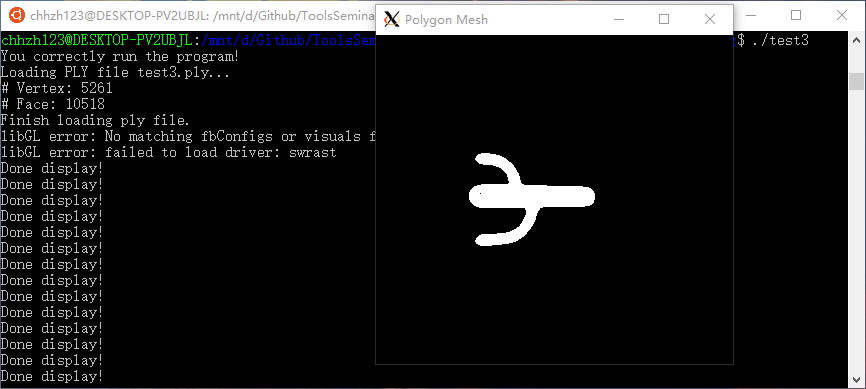
\includegraphics[width=\linewidth]{fig/assignments/autobuild_result.png}
\caption{Expected output: A cactus}
\label{fig:cactus}
\end{figure}

Several source program files are provided in \verb'Assignments/CppToolChain-AutoBuilding' folder, please \verb'cd' to that folder and have a look.\\
What you need to do is to \underline{\textbf{write a \emph{Makefile} or \emph{CMake} file}} to build the project and generate the expected results as shown above.
That is to say, you need NOT know how the program is working or how to use OpenGL.
You only need to glue these files together.

Firstly you should install some dependency libraries, which provide minimum support for graphical display.
Type the following commands on your Linux system.
\begin{lstlisting}
sudo apt-get update
sudo apt-get install freeglut3 freeglut3-dev
\end{lstlisting}

After installing the libraries above, you can begin your experiments.
To generate the output, you should follow the compilation and linking flow shown in Fig.~\ref{fig:autobuild}.
Since OOP and template are used, please use \verb'g++' to compile.
\begin{figure}[H]
\centering
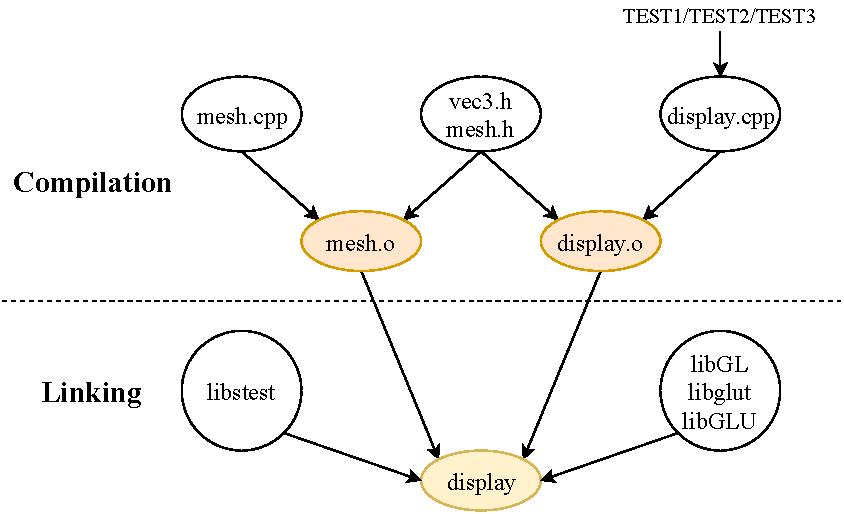
\includegraphics[width=0.8\linewidth]{fig/assignments/autobuild.pdf}
\caption{Compilation and linking flow}
\label{fig:autobuild}
\end{figure}

\verb'mesh.cpp' and \verb'display.cpp' are in the current folder.
\verb'vec3.h' and \verb'mesh.h' are in \verb'include/'.
\verb'libstest.a' is provided in \verb'lib/' folder.
\verb'libGL', \verb'libglut', and \verb'libGLU' has been installed by \verb'freeglut3' you just typed.
\verb'test1.in', \verb'test2.in', and \verb'test3.in' are three input files for the executable program.
Thus, you only need to generate the colored three files in Fig.~\ref{fig:autobuild}.
Detailed descriptions as follow:
\begin{enumerate}
\item Compile \verb'mesh.cpp' (which has included the \verb'mesh.h' and \verb'vec3.h' header) to \verb'mesh.o'.\\
(Hint: \verb'-c' flag enables \verb'g++' to compile the source file to the object file.)
\item Compile \verb'display.cpp' (which also includes the \verb'mesh.h' and \verb'vec3.h' header) to \verb'display.o'.
Notice three different macros (\verb'TEST1'/\verb'TEST2'/\verb'TEST3') should be defined respectively, which can be viewed in Line 190-196 in \verb'display.cpp'.\\
(Hint: \verb'-D' flag enables \verb'g++' to pass predefined macros to preprocessors.)
\item Link the generated \verb'mesh.o' and \verb'display.o' with three CG libraries called \verb'libGL', \verb'libglut', and \verb'libGLU'.
Also, a test static library provided in \verb'lib/libstest.a' should also be linked.\\
(Hint: To link these static libraries, the first three characters \verb'lib' can be omitted. For example, to link libGL, you only need to write \verb'-lGL'.)
\end{enumerate}

Basically, you will have three different \verb'display.o' files respectively for test1, test2, and test3, and one \verb'mesh.o' for all these tests.
For example, for test1, you define \verb'TEST1' when compiling \verb'display.cpp', generate \verb'display1.o', and obtain \verb'display1' executable, which reads in \verb'test1.obj' and outputs results.

If you correctly compile and link the files, you can run the generated \verb'display' programs and see \emph{three} different things displayed on the screen.
If you see that, cheers! You have done it!

\bigskip

I believe you will meet lots of problems in this project, so I list a few below:
\begin{enumerate}
	\item [Q1:] Compile time error
	\item [A1:] Maybe your \verb'g++' is out-of-date (use \verb'g++ --version' to check your version), please use the following commands to update your \verb'g++' (my Ubuntu system uses \verb'g++' 7.4.0 version) and change the default \verb'g++' version.
\begin{lstlisting}
sudo apt-get update
sudo apt-get install gcc-7 g++-7
sudo update-alternatives --config g++
\end{lstlisting}

	\item [Q2:] 
\fbox{\begin{minipage}{\linewidth}
\begin{flushleft}
display.cpp:10:10: \textcolor{red}{fatal error:} mesh.h: No such file or directory\\
 \#include \textcolor{red}{$<$mesh.h$>$}
\end{flushleft}
\end{minipage}}
	\item [A2:] Please check whether you correctly add include file search path in your command.\\
	(Hint: Use \verb'-I' command.)

	\item [Q3:]
\fbox{\begin{minipage}{\linewidth}
\begin{flushleft}
display.o: In function `init()':\\
display.cpp:(.text+0x1d): undefined reference to `glClearColor'\\
display.cpp:(.text+0x707): undefined reference to `gluPerspective'\\
display.o: In function `main':\\
display.cpp:(.text+0x944): undefined reference to `libTest()'\\
display.cpp:(.text+0x979): undefined reference to `glutInit'\\
collect2: \textcolor{red}{error}: ld returned 1 exit status
\end{flushleft}
\end{minipage}}
	\item [A3:] Please check if you link the three CG libraries (libGL, libglut, libGLU) and the test library (libstest) correctly.

	\item [Q4:] 
\fbox{\begin{minipage}{\linewidth}
\begin{flushleft}
/usr/bin/ld: cannot find -lstest\\
collect2: \textcolor{red}{error}: ld returned 1 exit status
\end{flushleft}
\end{minipage}}
	\item [A4:] Check if you add \verb'lib' to the link file search path.\\
	(Hint: Use \verb'-L' command.)

	\item [Q5:]
\fbox{\begin{minipage}{\linewidth}
\begin{flushleft}
\textcolor{red}{Error}: You do not load any models!
\end{flushleft}
\end{minipage}}
	\item [A5:] Please check if you define any one of the macros (\verb'TEST1', \verb'TEST2', \verb'TEST3') when compilation.

	\item [Q6:]
\fbox{\begin{minipage}{\linewidth}
\begin{flushleft}
Loading PLY file test3.ply...\\
\# Vertex: 5261\\
\# Face: 10518\\
Finish loading ply file.\\
You correctly run the program!\\
freeglut (./test3): failed to open display ''
\end{flushleft}
\end{minipage}}
	\item [A6:] This is good! You have done this project! This may result from your Linux system having no GUI. If you use WSL and insist to see the output figure, you can follow \href{https://virtualizationreview.com/articles/2017/02/08/graphical-programs-on-windows-subsystem-on-linux.aspx}{this page} to obtain your results.

	\item [Q7:] For any other questions, please Google or directly consult me.
\end{enumerate}

Moreover, about compiling and linking files in this tree-like structure, you can find more guidance on ECE 2400's \href{https://cornell-ece2400.github.io/ece2400-docs/ece2400-sec2-c-basics/}{webpage}.

\bigskip
To submit your homework, you need to \verb'git push' the whole \verb'CppToolchain-AutoBuilding' folder.
But remember to remove unnecessary files like \verb'mesh.o' and \verb'display.o' before you commit.

\subsection{Debugging}
Use \verb'gdb' or other debugging tools to find the bugs in the\\
\verb'Assignments\CppToolchain-Debugging\mergesort.c' program.

For details about the merge sort, you can refer to \href{https://www.geeksforgeeks.org/merge-sort/}{GeeksforGeeks}.

\end{document}